\documentclass{article}

% If you're new to LaTeX, here's some short tutorials:
% https://www.overleaf.com/learn/latex/Learn_LaTeX_in_30_minutes
% https://en.wikibooks.org/wiki/LaTeX/Basics

% Formatting
\usepackage[utf8]{inputenc}
\usepackage[margin=1in]{geometry}
\usepackage[titletoc,title]{appendix}


% Math
% https://www.overleaf.com/learn/latex/Mathematical_expressions
% https://en.wikibooks.org/wiki/LaTeX/Mathematics
\usepackage{amsmath,amsfonts,amssymb,mathtools}

% Images
% https://www.overleaf.com/learn/latex/Inserting_Images
% https://en.wikibooks.org/wiki/LaTeX/Floats,_Figures_and_Captions
\usepackage{graphicx,float}
\usepackage{pdfpages}
\usepackage{subcaption}

% Tables
% https://www.overleaf.com/learn/latex/Tables
% https://en.wikibooks.org/wiki/LaTeX/Tables

% Algorithms
% https://www.overleaf.com/learn/latex/algorithms
% https://en.wikibooks.org/wiki/LaTeX/Algorithms
\usepackage[ruled,vlined]{algorithm2e}
\usepackage{algorithmic}

% Code syntax highlighting
% https://www.overleaf.com/learn/latex/Code_Highlighting_with_minted
\usepackage{minted}
\usemintedstyle{borland}

% References
% https://www.overleaf.com/learn/latex/Bibliography_management_in_LaTeX
% https://en.wikibooks.org/wiki/LaTeX/Bibliography_Management
\usepackage[backend=biber, style=authoryear]{biblatex}
\addbibresource{myBibliography.bib}

% Title content
\title{AMATH 582 Homework 3}
\author{Daniel Burnham (https://github.com/burnhamdr)}
\date{February 21, 2020}

\begin{document}

\maketitle

% Abstract
\begin{abstract}
The work presented here is motivated by material covered in AMATH 582 Computational Methods For Data Analysis regarding the applications of Singular Value Decomposition (SVD). SVD is a linear algebra matrix factorization method that represents how the matrix of interest stretches/compresses and rotates a given set of vectors. The SVD is a powerful tool because the constitutive components of its factorization allow for the subsequent projection of a matrix onto low-dimensional representations. In the problem addressed here this is used to determine axes of motion of a spring-mass pendulum system from three different camera perspectives. Each camera records the action of the pendulum in a coordinate system relative to the camera which does not allow for complete characterization of the motion of the pendulum system from any one perspective. Gathering together positional information from each camera recording and applying SVD allows for the data matrix to subsequently be projected onto a low-dimensional space representing the axes where the most motion is detected in each camera. Principal Component Analysis (PCA) is the method used for this purpose and is an analysis concerned with the diagonalization and thus the dimensionality reduction of the covariance matrix of a system. The diagonalization in this instance will be performed using SVD allowing for the removal of redundancies and extraction of an ordered list of the axes of largest measurement variances (principal components). The experiments described in this work will describe PCA in more detail through practical application.
\end{abstract}

% Introduction and Overview
\section{Introduction and Overview}
The problem addressed here involves the analysis of data from three different cameras recording video perspectives of a spring-mass pendulum system. From this camera data the behavior of the system is described and the governing equations of motion determined. This analysis required work in two main categories: 1) Determining the position of the pendulum in each video frame for each camera 2) Applying PCA to position data from all camera perspectives to capture system dynamics. Three distinct cases of pendulum tracking and subsequent dynamics extraction will occur:
\begin{enumerate}
    \item (Test 1) Ideal Case: Small displacement of the pendulum mass in the z direction. In this case, the entire motion is in the z direction.
    \item (Test 2) Noisy Case: Repeat of the ideal case experiment, but in this case camera shake introduces noise to the video recording.
    \item (Test 3) Horizontal Displacement Case: In this experiment, the pendulum mass is released off-center so as to produce motion in the xy plane as well as the z direction.
    \item (Test 4) Horizontal Displacement and Rotation Case: In this experiment, the mass is released off-center and rotates so as to produce motion in the xy plane, rotation as well as the z direction.
\end{enumerate}

%  Theoretical Background
\section{Theoretical Background}
\subsection{Singular Value Decomposition (SVD)}\label{svdTheory}
SVD is a linear algebra method for factorization of a matrix into a number of constitutive components. It is rooted in the observation that during matrix vector multiplication of a vector $\mathbf{x}$ by a matrix $\mathbf{A}$ the resulting vector $\mathbf{y}$ has a new magnitude and direction. This transformation of the vector $\mathbf{x}$ by a matrix $\mathbf{A}$ implies that perhaps the action of matrix $\mathbf{A}$ can be replicated through component matrices that perform the same magnitude and direction manipulations. Furthermore, it would be beneficial if these components possessed properties that made them easy to work with, such as orthogonality and diagonality. The SVD factorization of the matrix $\mathbf{A}$ achieves these goals by expanding this observation of vector transformation under multiplication by a matrix to $\mathbb{R}^{m}$. SVD does this by building from the observation that the image of a unit sphere under any m$\times$n matrix is a hyperellipse. This can be visualized more clearly in Figure~\ref{fig:hype}. Following from this, one can represent this transformation as $\mathbf{A}\mathbf{v}_{j} = \sigma_{j}\mathbf{u}_{j}$ for $1\leq j\leq n$. Where $\mathbf{v}_{j}$ are the vectors of the unit sphere transformed by $\mathbf{A}$, and $\sigma_{j}\mathbf{u}_{j}$ are the resulting transformations representing the the semiaxes of the hyperellipse. Rearranging this equation allows for the SVD factorization of $\mathbf{A}$ to be written as follows (\cite{kutz_2013}):
\begin{equation}\label{eq:svd}
\mathbf{A}= \mathbf{U}\boldsymbol{\Sigma} \mathbf{V}^*
\end{equation}
In this form, $\mathbf{U}$ is unitary and contains the vectors $\mathbf{u}_{j}$ indicating the directions of the transformed hyperellipse semiaxes, $\boldsymbol{\Sigma}$ is diagonal and contains the scaling values corresponding to these semiaxes, and $\mathbf{V}^{*}$ is the Hermitian transpose of $\mathbf{V}$ which contains the orthonormal basis of the vectors that are transformed under $\mathbf{A}$.
\begin{figure}[t]
    \centering
    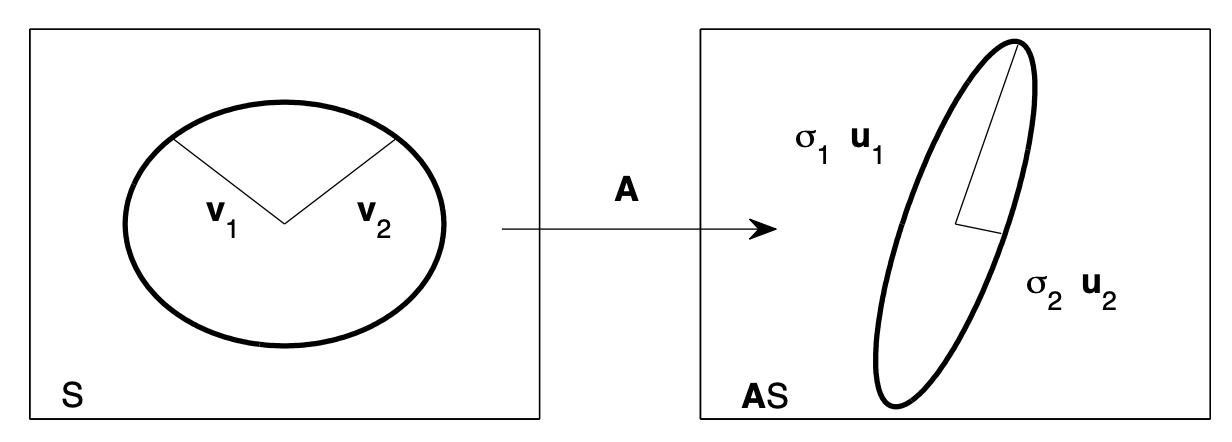
\includegraphics[width=0.435\linewidth]{Screen Shot 2020-02-25 at 10.05.25 AM.png}
    \caption{Image of a unit sphere $\mathit{S}$ transformed into a hyperellipse $\mathbf{A}\mathit{S}$ in $\mathbb{R}^{n}$. The values of $\sigma1$ and $\sigma2$ are the singular values of the matrix $\mathbf{A}$ and represent the lengths of the semiaxes of the ellipse. (\cite{kutz_2013})}
    \label{fig:hype}
\end{figure}
It is worth noting that it can be proved that every matrix $\mathbf{A}\in\mathbb{C}^{m\times n}$ has a singular value decomposition and the singular values are uniquely determined (\cite{kutz_2013}). Additionally, if the matrix $\mathbf{A}$ is square, the singular vectors $\mathbf{u}_{j}$ and $\mathbf{v}_{j}$ are also uniquely determined up to complex signs (\cite{kutz_2013}). This is significant because it allows for every $\mathbf{A}\in\mathbb{C}^{m\times n}$ to be factorized by SVD and subsequently represented with lower rank matrix approximations. This will be useful in the context of the pendulum problem explored here as it represents a way of reducing the dimensionality of the pendulum positional data.

\subsection{Principal Component Analysis (PCA)}
PCA is a variant of SVD that is motivated by finding low-dimensional reduction of information from seemingly complex data. In the context of the experiments investigated in this report, this complex data is the pendulum positions recorded for each video frame captured by the perspective of each camera. The intuition for PCA builds from the identification of two characteristics of complex data sets: noise and redundancy. Noise in the data has the potential to obscure meaningful information represented by the data. Redundancy in the data refers to data observations that overlap in that they contribute to describing variance along the same dimension of the overall data. Addressing this redundancy is critical for data analysis and relies on the covariance matrix of the data. Covariance measures the statistical dependence or independence between two variables. The covariance matrix of a set of data $\mathbf{X}$ with itself will elucidate which observations within the dataset are redundant, or in other words, how much each observational measurement correlates with measurements of other observations of the dataset. This covariance matrix is thus defined as (\cite{kutz_2013}):
\begin{equation}\label{eq:cov}
\mathbf{C}_{\mathbf{X}} = \frac{1}{n-1}\mathbf{X}\mathbf{X^{\mathit{T}}}
\end{equation}
The covariance matrix $\mathbf{C}_{\mathbf{X}}$ is square and symmetric with diagonal entries that represents the variance of of each observation. The off-diagonal terms are the covariances between observations. In this way, the covariance matrix represents how each observation correlates with every other observation in the data. Redundancies within the data are thus identifiable by off-diagonal terms, as large off-diagonal values indicate a high degree of correlation (redundancy) while the opposite is true for small off-diagonal values. The diagonal terms are of particular interest because large values here indicate a high degree of variance within a particular observation thus indicating a variable of potential interest in driving differentiation in output variables. In the case of the pendulum system investigated in this report, this output variable is position, and the observations are the x and y position data from each camera. A large diagonal term for this data matrix would thus indicate a dimension of a specific camera perspective that captures a significant portion of the pendulum system dynamics. The goal of PCA is to then take this covariance matrix and extract the most interesting descriptions of the underlying data. This is accomplished by diagonalizing the covariance matrix because through diagonalization the correct coordinate system relative to the data is determined and can be used to reduce the dimensionality of the data. SVD presents as a promising candidate for diagonalizing the covariance matrix. As discussed in Section~\ref{svdTheory} the SVD factorizes a matrix $\mathbf{A}$ into two sets of bases and a diagonal matrix. One way of conceptualizing this factorization is that the orthonormal bases $\mathbf{U}$ and $\mathbf{V}$ are the bases that diagonalize the matrix $\mathbf{A}$. The mathematical foundation of PCA begins with this conceptualization in order to diagonalize the covariance matrix. In order to find the appropriate bases for this diagonalization, the first step is to define a transformed variable $\mathbf{Y}$ as $\mathbf{Y} = \mathbf{U}^*\mathbf{X}$ where $\mathbf{U}$ is the unitary transformation associated with the SVD of $\mathbf{X}$ (Equation~\ref{eq:svd}). From this, the variance in $\mathbf{Y}$ can be calculated as follows (\cite{kutz_2013}):
\begin{equation}\label{eq:covy}
\begin{aligned}
\mathbf{C}_{\mathbf{Y}} &= \frac{1}{n-1}\mathbf{Y}\mathbf{Y^{\mathit{T}}} \\
& = \frac{1}{n-1}(\mathbf{U^{*}X})(\mathbf{U^{*}X})^{\mathit{T}} \\
& = \frac{1}{n-1}\mathbf{U^{*}}(\mathbf{XX}^{\mathit{T}})\mathbf{U} \\
& = \frac{1}{n-1}\mathbf{U^{*}}\mathbf{U}\boldsymbol{\Sigma}^{2}\mathbf{UU^{*}} \\
& = \frac{1}{n-1}\boldsymbol{\Sigma}^{2}
\end{aligned}
\end{equation}
Through this diagonalization the ideal basis is found in which the covariance matrix $\mathbf{C}_{X}$ can be represented such that redundancies are removed, and the largest variances of particular observations are ordered. More specifically, the basis formed by the left singular vectors of $\mathbf{X}$ (the columns of $\mathbf{U}$) is the ideal basis in which to express $\mathbf{X}$ such that the covariance matrix ($\mathbf{C}_{X}$) is diagonal. The largest diagonal entries of $boldsymbol{\Sigma}$ thus correspond to the directions of largest variance of $\mathbf{X}$.

% Algorithm Implementation and Development
\section{Algorithm Implementation and Development}
The main steps of the algorithm are as follows: 
\begin{enumerate}
    \item Input the video file, prepare for analysis
    \item For each camera locate paint can pendulum in each video frame
    \item Collect positional data from each camera and perform PCA
    \item Plot dynamics along the principal component directions by video frame for each test case to visualize the dynamics of the spring-mass pendulum system.
\end{enumerate}

\subsection{Pendulum Position Detection}
The nature of the recorded videos presents a challenge in reliably detecting the paint can (the pendulum mass) in each video frame. In order to address this challenge some image processing techniques are employed based on observational evidence. Firstly, the pendulum oscillates largely in the foreground of the video allowing for foreground filtering (Otsu's method) to limit the interference of the background. Secondly, a high pass filter helps to emphasize objects in the foreground that have edges, such as the paint can pendulum. These two image processing methods allow for the white pixel features of the paint can to be made the most prominent feature of each video frame. After this preprocessing, a search window is subsequently iterated across each video frame searching for the windowed portion of the video frame with the highest average pixel value. The robustness of the preprocessing methods allow for the location of this window within the frame to reliably represent the position of the paint can.

\begin{algorithm}
\begin{algorithmic}
    \STATE{Determine shape of data matrix (i.e. width and height of individual frames, and number of video frames)}
    \FOR{each video frame}
        \STATE{convert video frame to grayscale}
        \STATE{apply otsu foreground filter to band of pixels around the edge of the frame}
        \STATE{apply high-pass filter to foreground filtered grayscale video frame}
        \FOR{each x pixel coordinate}
            \FOR{each y pixel coordinate}
                \IF{pixel value $>$ threshold} 
                    \STATE{set pixel value to maximum value (255)}
                \ELSE
                    \STATE{set pixel value to zero}
                \ENDIF
            \ENDFOR
        \ENDFOR
        \FOR{each x pixel coordinate within search window}
            \FOR{each y pixel coordinate within search window}
                \STATE{calculate average pixel value}
                \IF{average pixel value $>$ max average pixel value} 
                    \STATE{set position of maximum average pixel value to the current location in pixel space of the upper left corner pixel of the search window}
                \ELSE
                    \STATE{keep previous position of maximum average pixel value}
                \ENDIF
            \ENDFOR
        \ENDFOR
        \STATE{add position of maximum pixel value to list of positions tracking the pendulum position across all video frames}
    \ENDFOR

\end{algorithmic}
\caption{Track Pendulum Position}
\label{alg:penPos}
\end{algorithm}

% Computational Results
\section{Computational Results}
\begin{figure}
\centering
   \begin{subfigure}{0.49\linewidth} \centering
     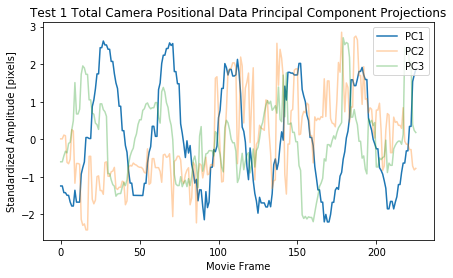
\includegraphics[scale=0.5]{T1_pcDynamics.png}
   \end{subfigure}
   \begin{subfigure}{0.49\linewidth} \centering
     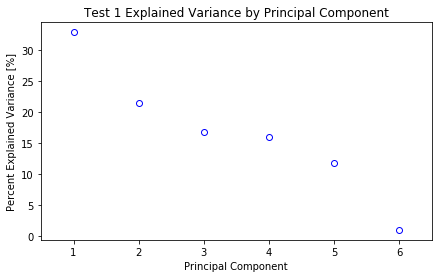
\includegraphics[scale=0.5]{T1_pcExplainedVariance.png}
   \end{subfigure}
\caption{(Left) Plot of the principal component projections of the camera positional data for the top three principal components across the video frames recorded. (Right) Plot of the explained variance along each principal component} \label{fig:test1}
\end{figure}
\begin{figure}
\centering
   \begin{subfigure}{0.49\linewidth} \centering
     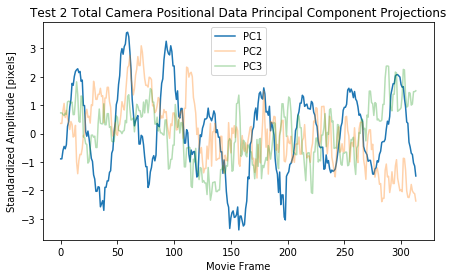
\includegraphics[scale=0.5]{T2_pcDynamics.png}
   \end{subfigure}
   \begin{subfigure}{0.49\linewidth} \centering
     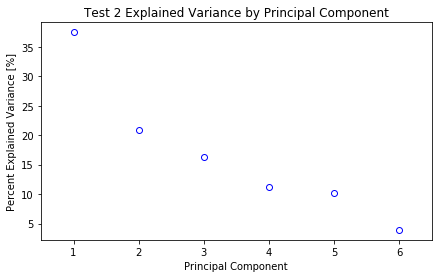
\includegraphics[scale=0.5]{T2_pcExplainedVariance.png}
   \end{subfigure}
\caption{(Left) Plot of the principal component projections of the camera positional data for the top three principal components across the video frames recorded. (Right) Plot of the explained variance along each principal component} \label{fig:test2}
\end{figure}
\begin{figure}
\centering
   \begin{subfigure}{0.49\linewidth} \centering
     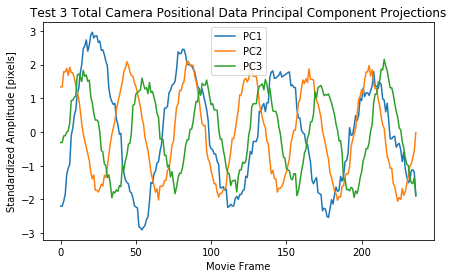
\includegraphics[scale=0.5]{T3_pcDynamics.png}
   \end{subfigure}
   \begin{subfigure}{0.49\linewidth} \centering
     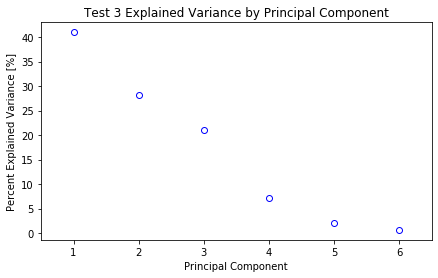
\includegraphics[scale=0.5]{T3_pcExplainedVariance.png}
   \end{subfigure}
\caption{(Left) Plot of the principal component projections of the camera positional data for the top three principal components across the video frames recorded. (Right) Plot of the explained variance along each principal component} \label{fig:test3}
\end{figure}
\begin{figure}
\centering
   \begin{subfigure}{0.49\linewidth} \centering
     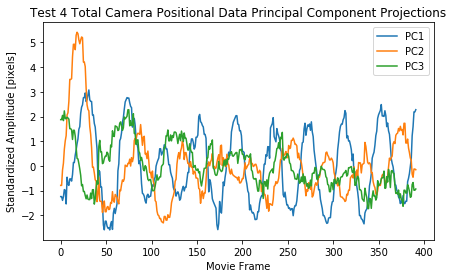
\includegraphics[scale=0.5]{T4_pcDynamics.png}
   \end{subfigure}
   \begin{subfigure}{0.49\linewidth} \centering
     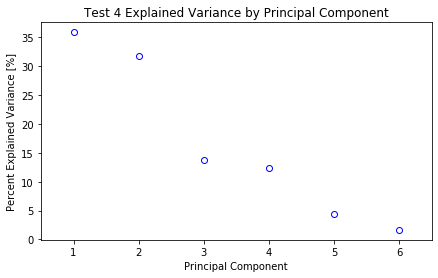
\includegraphics[scale=0.5]{T4_pcExplainedVariance.png}
   \end{subfigure}
\caption{(Left) Plot of the principal component projections of the camera positional data for the top three principal components across the video frames recorded. (Right) Plot of the explained variance along each principal component} \label{fig:test4}
\end{figure}

\subsection{Test 1: Simple Harmonic Oscillations}
See Figure~\ref{fig:test1} for the results of applying PCA to the positional data returned by Algorithm~\ref{alg:penPos}. Oscillations are evident along a single dimension. These observed system dynamics are supported by the percent explained variance of the first principal component individually representing roughly a third of the overall variance of the system. The rest of the variance observed is attributable to noise based on the nature of the dynamics illustrated by the projections of the data along the second and third principal components. These findings are consistent with the conditions posed for test 1 where the entire motion of the spring-mass pendulum system was restricted to the z directions with the goal of observing simple harmonic motion.

\subsection{Test 2: Simple Harmonic Oscillations with Noise}
See Figure~\ref{fig:test2} for the results of applying PCA to the positional data returned by Algorithm~\ref{alg:penPos}. Oscillations are evident along a single dimension. These observed system dynamics are supported by the percent explained variance of the first principal component individually representing over 35 percent of the overall variance of the system. The rest of the variance observed is attributable to noise (similarly to test 1) based on the nature of the dynamics illustrated by the projections of the data along the second and third principal components. These findings are consistent with the conditions posed for test 2 where the entire motion of the spring-mass pendulum system was restricted to the z direction, but noise in the form of camera shake was introduced to the video recordings. Simple harmonic motion remains evident in projecting the data along the first principal component.

\subsection{Test 3: Horizontal Pendulum Motion and Simple Harmonic
Oscillations}
See Figure~\ref{fig:test3} for the results of applying PCA to the positional data returned by Algorithm~\ref{alg:penPos}. Oscillations are evident along a three dimensions. These observed system dynamics are supported by the percent explained variance of the first, second, and third principal components individually representing approximately 40, 30, and 20 percent of the overall variance of the system respectively. The rest of the variance observed is attributable to noise. These findings are consistent with the conditions posed for test 3 where the motion of the spring-mass pendulum system should occur in the x, y, and  z directions.

\subsection{Test 4: Horizontal Pendulum Motion and Simple Harmonic
Oscillations.. with a Twist}
See Figure~\ref{fig:test4} for the results of applying PCA to the positional data returned by Algorithm~\ref{alg:penPos}. Oscillations are evident along a three dimensions. These observed system dynamics are supported by the percent explained variance of the first, second, and third principal components individually representing approximately 35, 30, and 15 percent of the overall variance of the system respectively. The rest of the variance observed is attributable to noise. These findings are consistent with the conditions posed for test 4 where the motion of the spring-mass pendulum system should occur in the x, y, and  z directions. The rotation of the pendulum is not captured by the positional data and simply made tracking the pendulum between video frames more challenging.

% Summary and Conclusions
\section{Summary and Conclusions}
Overall a video processing algorithm was successfully developed for the extraction of positional data from three unique camera perspectives characterizing a spring-mass pendulum system. This algorithm was tunable allowing for reliable pendulum tracking in all test cases. PCA was successfully implemented to elucidate the dynamics of this physical system along the most relevant axes for each experimental test case.
% References
\printbibliography

% Appendices
\begin{appendices}

% Python Functions
\section{Python Functions}
\begin{itemize}
    \item \texttt{sklearn.decomposition.PCA(n\_components=None, copy=True, whiten=False, svd\_solver='auto', tol=0.0, iterated\_power='auto', random\_state=None)}\\ 
    Principal component analysis (PCA). Linear dimensionality reduction using Singular Value Decomposition of the data to project it to a lower dimensional space. The input data is centered but not scaled for each feature before applying the SVD. It uses the LAPACK implementation of the full SVD or a randomized truncated SVD by the method of Halko et al. 2009, depending on the shape of the input data and the number of components to extract. It can also use the scipy.sparse.linalg ARPACK implementation of the truncated SVD.
    \item \texttt{numpy.fft.fft2(a, s=None, axes=(-2, -1), norm=None)}\\ Compute the 2-dimensional discrete Fourier Transform.
    This function computes the n-dimensional discrete Fourier Transform over any axes in an M-dimensional array by means of the Fast Fourier Transform (FFT). By default, the transform is computed over the last two axes of the input array, i.e., a 2-dimensional FFT.
    \item \texttt{sklearn.preprocessing.StandardScaler(copy=True, with\_mean=True, with\_std=True)} \\
    Standardize features by removing the mean and scaling to unit variance
    \item \texttt{numpy.amax(a, axis=None, out=None, keepdims=<no value>, initial=<no value>, where=<no value>)} \\
    Return the maximum of an array or maximum along an axis.
    \item \texttt{skimage.filters.threshold\_otsu(image, nbins=256)}\\ Return threshold value based on Otsu’s method.
    
\label{itemize:functions}
\end{itemize}

% Python Code
\section{Python Code}
\inputminted{python}{HW3_DanielBurnham.py}
\label{appendix:code}

\end{appendices}



\end{document}